\documentclass[problem]{mcs}

\begin{pcomments}
  \pcomment{PS_coloring_no_triangles}
  \pcomment{by Diego C., edited by ARM 3/16}
\end{pcomments}

\pkeywords{
coloring
triangle-free
chromatic number
}

%%%%%%%%%%%%%%%%%%%%%%%%%%%%%%%%%%%%%%%%%%%%%%%%%%%%%%%%%%%%%%%%%%%%%
% Problem starts here
%%%%%%%%%%%%%%%%%%%%%%%%%%%%%%%%%%%%%%%%%%%%%%%%%%%%%%%%%%%%%%%%%%%%%

\begin{problem}
A basic example of a simple graph with chromatic number $n$ is the
complete graph on $n$ vertices, that is $\chi(K_n)=n$.  This implies
that any graph with $K_n$ as a subgraph must have chromatic number at
least $n$.  It's a common misconception to think that, conversely,
graphs with high chromatic number must contain a large complete
subgraph.  In this problem we exhibit a simple example countering this
misconception, namely a graph with chromatic number four that contains
no \emph{triangle}---length three cycle---and hence no subgraph
isomorphic to $K_n$ for $n \geq 3$.  Namely, let $G$ be the
$11$-vertex graph of Figure~\ref{fig:coloring_no_triangles}.  The
reader can verify that $G$ is triangle-free.

\bparts

\ppart Show that $G$ is 4-colorable.

\begin{solution}
  Figure \ref{fig:coloring_no_triangles_solution} shows a valid coloring.
\begin{figure}\inbook{[h]}
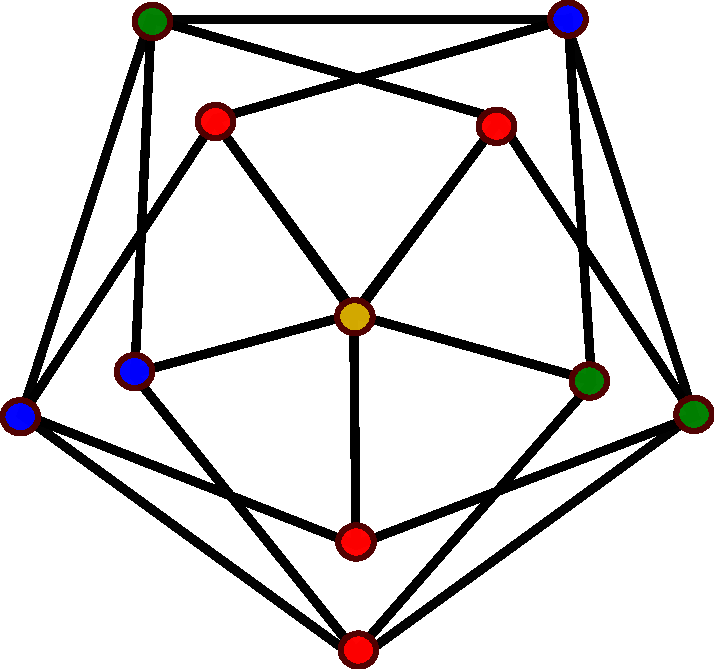
\includegraphics[width=2in]{coloring_no_triangles_solution}
\caption{Coloring using 4 colors}
\label{fig:coloring_no_triangles_solution}
\end{figure}
\end{solution}

\ppart Prove that $G$ can't be colored with $3$
colors.

%\examspace
%\instatements{\newpage}
\begin{figure}\inbook{[hb]}
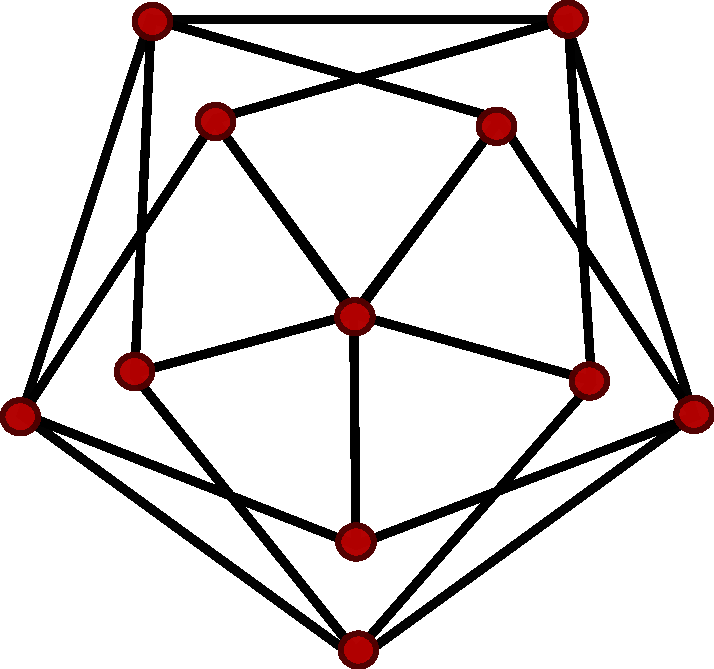
\includegraphics[width=1.6in]{coloring_no_triangles}
\caption{Graph $G$ with no triangles and $\chi(G)=4$.}
\label{fig:coloring_no_triangles}
\end{figure}


\begin{solution}
Assume by contradiction that there is one coloring using only 3
colors: red, blue and green.  The outer pentagon of the graph is an
odd-length cycle, and so requires all 3 colors.  So we can assume wlog
that the outer pentagon is colored as shown in the left hand side of
Figure \ref{fig:coloring_no_triangles_solution2}.

This coloring of the pentagon forces the coloring of three interior
points, as shown in the right hand side of Figure
\ref{fig:coloring_no_triangles_solution2}.  Now the point in the
center has neighbors with all three colors, so it is impossible to
color it.

\begin{figure}\inbook{[h]}
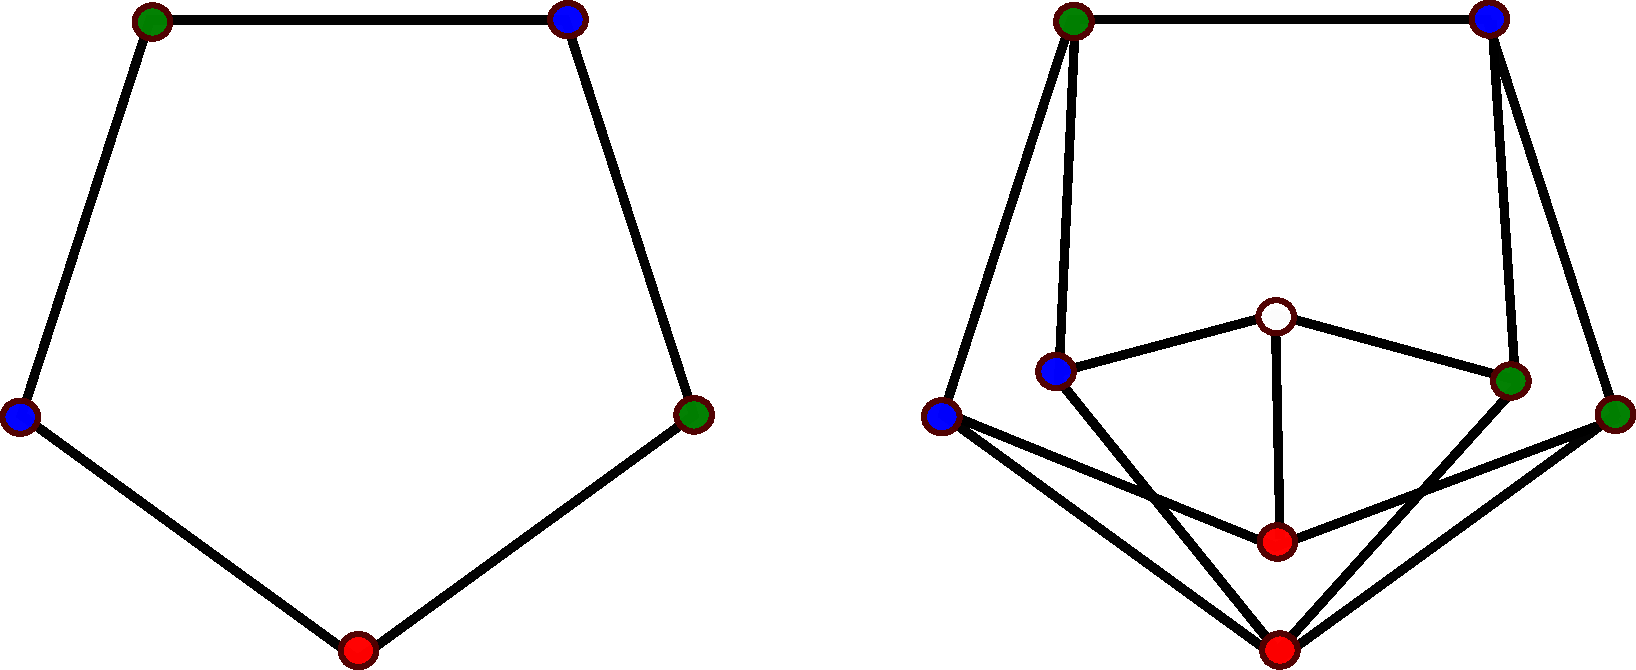
\includegraphics[width=4in]{coloring_no_triangles_solution2}
\caption{Constraints on a 3-coloring.}
\label{fig:coloring_no_triangles_solution2}
\end{figure}

The graph $G$ is the known as the \emph{Groetzsch graph}.  It is the
smallest triangle-free graph with chromatic number 4.  It turns out
that for any $n>0$, there is a triangle-free graph with chromatic
number $n$, see
\href{http://mathworld.wolfram.com/MycielskiGraph.html}{\emph{Mycielski
    graphs}} on the Wolfram Mathworld web site.
\end{solution}
\eparts

\end{problem}

%%%%%%%%%%%%%%%%%%%%%%%%%%%%%%%%%%%%%%%%%%%%%%%%%%%%%%%%%%%%%%%%%%%%%
% Problem ends here
%%%%%%%%%%%%%%%%%%%%%%%%%%%%%%%%%%%%%%%%%%%%%%%%%%%%%%%%%%%%%%%%%%%%%

\endinput
